\documentclass[10pt,letterpaper]{article}
\usepackage[top=0.75in,bottom=0.8in,left=0.9in,right=0.9in]{geometry}
\usepackage[T1]{fontenc}
\usepackage{times}
\renewcommand{\ttdefault}{lmtt}
\usepackage{microtype}
\usepackage{graphicx}
\usepackage{booktabs}
\usepackage[hidelinks]{hyperref}
\usepackage[font=small,labelfont=bf,labelsep=period]{caption}
\usepackage{titlesec}
\usepackage{tikz}
\usetikzlibrary{arrows.meta,positioning}
\tikzset{box/.style={draw,rounded corners=2pt,align=center,font=\footnotesize,inner sep=4pt,minimum height=0.95cm},arr/.style={-{Stealth[length=1.8mm]},semithick},lab/.style={font=\scriptsize,align=center}}

\titleformat{\section}{\large\bfseries}{\thesection}{0.6em}{}
\titlespacing*{\section}{0pt}{1.6ex plus .3ex}{0.8ex}
\setlength{\parskip}{0.3ex}
\renewcommand{\topfraction}{0.9}
\renewcommand{\bottomfraction}{0.8}
\renewcommand{\textfraction}{0.07}
\renewcommand{\floatpagefraction}{0.8}
\setlength{\textfloatsep}{8pt plus 2pt}
\setlength{\intextsep}{6pt plus 2pt}

\title{\vspace{-2.2em}\textbf{Painting with Darts: A Language-Conditioned\\Tool-Aiming Dataset for Low-Cost Robot Arms}\thanks{Dataset: \url{https://huggingface.co/datasets/vineethsendilraj/pi07-dart-painting-so101}. Code, wiring and training logs: \url{https://github.com/VineethSendilraj/pi07-dart-painting-so101}.}}
\author{Vineeth Sendilraj \qquad Vardhan Agnihotri \qquad Yuvraj Lakhotia\\[2pt]
\small Act-athon 2026, Actor Labs $\times$ Physical Intelligence (3rd place)}
\date{\vspace{-1.2em}}

\begin{document}
\maketitle

\begin{abstract}
\noindent
Open robot-learning datasets are dominated by grasping and pick-and-place. We release a dataset for a different class of skill: aiming a handheld, actuated tool at a language-specified target and triggering it. A low-cost SO-101 arm holds the handle of a motorized dart blaster and aims it at a cell of a 5$\times$5 grid given the instruction ``shoot $\langle$cell$\rangle$''. The dataset contains 116 teleoperated demonstrations (29{,}131 frames, 16 minutes at 30\,Hz) with two camera views, joint states, joint-space actions and a binary trigger channel, covering 23 targets, three levels of scene clutter, 17 start poses, and both live and dry shots. Because it differs from common manipulation data in embodiment, task structure and action space, it is suited as out-of-distribution data in training mixtures for generalist policies and as a small benchmark for language-conditioned precision aiming. Fine-tuning $\pi_{0.7}$ on it across 13 configurations, validation error is lowest after about 33 passes (0.287), and every probed checkpoint aims in the commanded row and column order. Combined with a vision-language model (VLM) that plans targets and verifies hits from images, the policy drew pictures with darts in a live demonstration. The data (LeRobot format, CC BY 4.0), code and wiring are public.
\end{abstract}

\section{Introduction}

Open robot-learning datasets mostly cover grasping and pick-and-place with a parallel gripper. Many practical skills instead involve holding a tool and pointing it, as in spraying, drilling or aiming a nozzle. These differ from grasping in three ways: success depends on the tool's orientation rather than on contact, the effect lands away from the robot, and the action combines continuous motion with a discrete actuation command. We collected a small dataset of this kind, in which an SO-101 arm aims a motorized dart blaster at a language-specified cell and fires it. We fine-tune the $\pi_{0.7}$ vision-language-action model~\cite{pi07} on these data and pair it with a VLM that plans targets and checks hits, a common hierarchy for long-horizon tasks~\cite{hirobot}, to draw pictures with darts.


\begin{figure}[!ht]
\centering
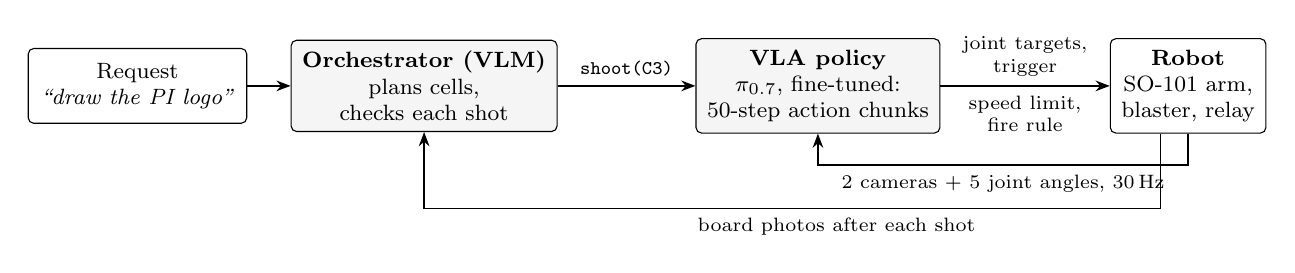
\begin{tikzpicture}
\node[box] (goal) {Request\\\textit{``draw the PI logo''}};
\node[box, fill=black!4, right=0.55cm of goal] (llm) {\textbf{Orchestrator (VLM)}\\plans cells,\\checks each shot};
\node[box, fill=black!4, right=1.75cm of llm] (vla) {\textbf{VLA policy}\\$\pi_{0.7}$, fine-tuned:\\50-step action chunks};
\node[box, right=2.15cm of vla] (robot) {\textbf{Robot}\\SO-101 arm,\\blaster, relay};
\draw[arr] (goal) -- (llm);
\draw[arr] (llm) -- node[lab, above] {\texttt{shoot(C3)}} (vla);
\draw[arr] (vla) -- node[lab, above] {joint targets,\\trigger} node[lab, below] {speed limit,\\fire rule} (robot);
\draw[arr] (robot.south) -- ++(0,-0.4) -| node[lab, pos=0.25, below] {2 cameras + 5 joint angles, 30\,Hz} (vla.south);
\draw[arr] (robot.south) ++(-0.35,0) -- ++(0,-0.95) -| node[lab, pos=0.22, below] {board photos after each shot} (llm.south);
\end{tikzpicture}
\caption{System overview. The VLM decides which cell to shoot next and verifies the result from photographs; the fine-tuned $\pi_{0.7}$ policy turns each \texttt{shoot(cell)} command and the live camera stream into joint targets and a trigger at 30\,Hz.}
\label{fig:system}
\end{figure}

\section{Setup}

\begin{figure}[!ht]
  \centering
  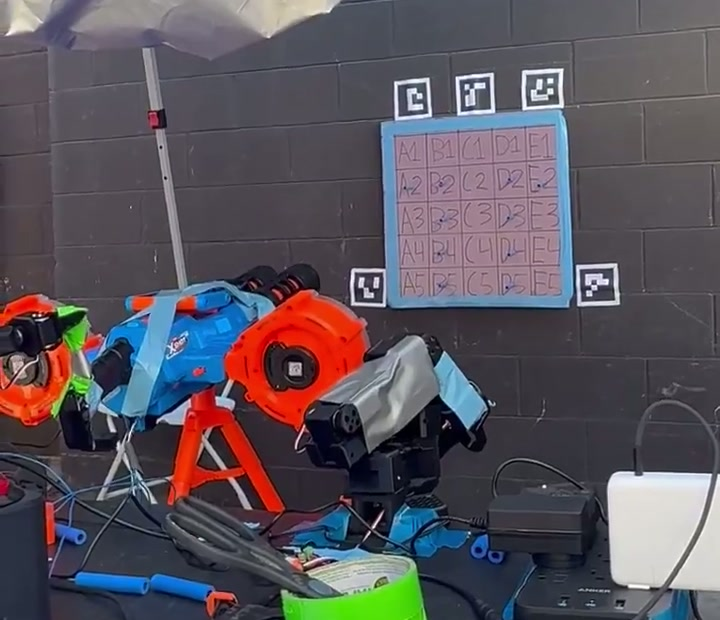
\includegraphics[height=2.9cm]{figs/rig.jpg}\hspace{4pt}%
  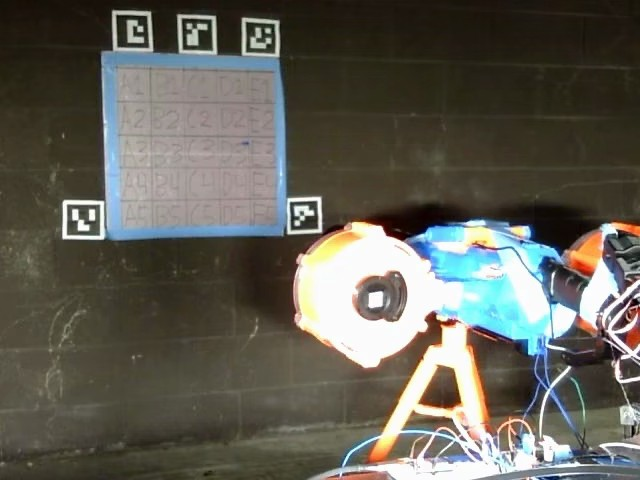
\includegraphics[height=2.9cm]{figs/front.jpg}\hspace{4pt}%
  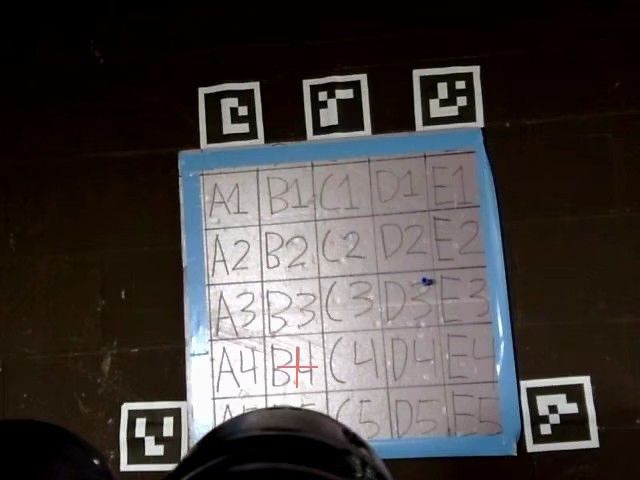
\includegraphics[height=2.9cm]{figs/wrist.jpg}
  \caption{Left: the rig. Middle and right: the policy's rear and blaster-mounted cameras during a \texttt{shoot B4} demonstration; the red cross marks the barrel axis.}
  \label{fig:rig}
\end{figure}

The follower arm's gripper is replaced by a wire loop around the blaster handle, and an ESP32-driven relay replaces the blaster's trigger switch, so firing is a binary action (Fig.~\ref{fig:rig}); Fig.~\ref{fig:system} shows the control loop. The policy observes two 640$\times$480 images (a rear view of the arm and board, and a view from the blaster) and five joint angles at 30\,Hz. It outputs chunks of 50 future steps, each with five absolute joint targets and a trigger value. At inference we execute 25 steps per chunk, limit each joint to $3^\circ$ per step, and fire once the arm is still and the predicted trigger has exceeded 0.5 for three consecutive steps.

Above the policy, a general-purpose VLM receives the requested picture and photographs from both cameras, and issues one \texttt{shoot(cell)} command at a time. After each shot it receives new photographs, so a dart that missed or fell out is detected and the cell is shot again.

\section{Dataset}

An operator aimed the follower with a leader arm and fired with a physical button, while a web application proposed the next cell, board clutter and start pose and replayed each take for keep-or-discard review (Fig.~\ref{fig:pipeline}). Each kept frame holds both images, five follower joint angles, and an action of five leader joint angles plus a trigger that is 1 for the 10 steps after the button press. A5 and E5 were not recorded.

\begin{figure}[!ht]
\centering
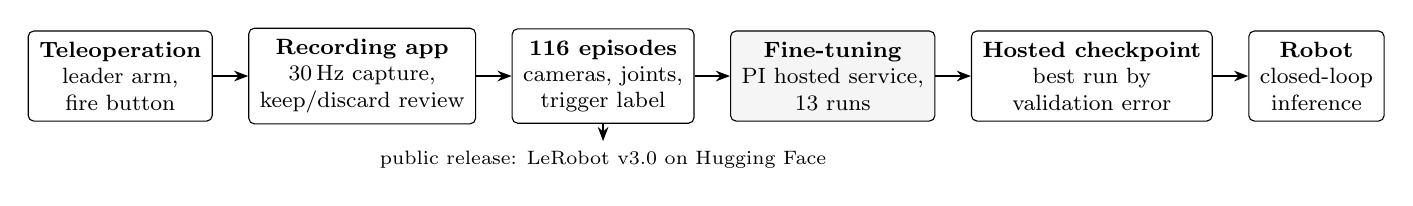
\begin{tikzpicture}
\node[box] (tele) {\textbf{Teleoperation}\\leader arm,\\fire button};
\node[box, right=0.45cm of tele] (rec) {\textbf{Recording app}\\30\,Hz capture,\\keep/discard review};
\node[box, right=0.45cm of rec] (eps) {\textbf{116 episodes}\\cameras, joints,\\trigger label};
\node[box, fill=black!4, right=0.45cm of eps] (ft) {\textbf{Fine-tuning}\\PI hosted service,\\13 runs};
\node[box, right=0.45cm of ft] (ckpt) {\textbf{Hosted checkpoint}\\best run by\\validation error};
\node[box, right=0.45cm of ckpt] (inf) {\textbf{Robot}\\closed-loop\\inference};
\node[lab, below=0.22cm of eps] (hf) {public release: LeRobot v3.0 on Hugging Face};
\draw[arr] (tele) -- (rec); \draw[arr] (rec) -- (eps); \draw[arr] (eps) -- (ft);
\draw[arr] (ft) -- (ckpt); \draw[arr] (ckpt) -- (inf); \draw[arr] (eps) -- (hf);
\end{tikzpicture}
\caption{Data and training pipeline. The same episodes are exported to LeRobot format for public release.}
\label{fig:pipeline}
\end{figure}

\section{Training and Results}

We ran 13 fine-tuning jobs on Physical Intelligence's hosted service, varying the training schedule, batch size, data mixture and base checkpoint (Table~\ref{tab:runs}). The training schedule mattered most: validation error was lowest after about 33 passes over the data on the standard base checkpoint and about 18 passes on an alternative base, and longer training overfit. A larger batch and oversampling the cells of the PI logo did not help, and training only on the 101 takes recorded with the final crosshair overlay was no better than using all 116. The run with the lowest error on the standard base was used for the live demonstration.

\begin{table}[!ht]
\centering\footnotesize\renewcommand{\arraystretch}{0.95}
\caption{Validation error of all 13 fine-tuning runs (best checkpoint per run), by base checkpoint.}
\label{tab:runs}
\begin{tabular}{@{}lcc@{}}
\multicolumn{3}{c}{\textit{Standard base}}\\
\toprule
Change from baseline & Passes & Val.\ error \\
\midrule
None (baseline) & 26.5 & 0.298 \\
\textbf{Longer schedule (demo)} & 33.5 & \textbf{0.287} \\
Much longer schedule & 48.5 & 0.303 \\
Batch size 512 & 48.5 & 0.334 \\
Logo cells oversampled & 33.5 & 0.333 \\
Final-crosshair takes only & $\sim$47 & 0.325$^{a}$ \\
Still frames dropped & 26.5 & 0.421$^{b}$ \\
\bottomrule
\end{tabular}\hspace{1.2em}%
\begin{tabular}{@{}lcc@{}}
\multicolumn{3}{c}{\textit{Alternative base}}\\
\toprule
Change from baseline & Passes & Val.\ error \\
\midrule
None & 26.5 & 0.294 \\
Shorter schedule & 17.6 & 0.294 \\
Logo cells oversampled & 17.6 & 0.281$^{c}$ \\
Final-crosshair takes only & $\sim$47 & 0.294$^{a}$ \\
Still frames dropped & 17.6 & 0.375$^{b}$ \\
Logo + still frames dropped & 17.6 & 0.444$^{b}$ \\
\addlinespace[1.05em]
\bottomrule
\end{tabular}\\[3pt]
\parbox{0.92\textwidth}{\footnotesize $^{a}$Validated on the 101-take subset. $^{b}$Validated on moving frames only. $^{c}$The validation split likely over-represents the logo cells. Scores marked $a$--$c$ are not directly comparable with the others.}
\end{table}

To test whether the policy uses the instruction, we gave each checkpoint the same images and joint state while changing only the cell in the prompt. All 24 probed checkpoints produced aims ordered by column and row, so the policy follows the instruction rather than replaying a fixed motion.

\section{Limitations}

We did not measure a hit rate on the real system; our evidence is validation error, the prompt probe and the live demonstration. Because each demonstration continues for 2\,s after the shot with the trigger at 0, the policy rarely produced a clean trigger pulse offline; the stillness rule in Section~2 compensates. Coverage is uneven (two demonstrations each for row~1, A3 and E3), and the camera and board positions were fixed throughout.


\footnotesize\raggedright
\renewcommand{\refname}{\normalsize References}
\begin{thebibliography}{3}
\setlength{\itemsep}{1pt}
\bibitem{pi07} Physical Intelligence. $\pi_{0.7}$: A steerable generalist robotic foundation model with emergent capabilities. arXiv:2604.15483, 2026.
\bibitem{hirobot} L.~X.~Shi, B.~Ichter, M.~Equi, et al. Hi Robot: Open-ended instruction following with hierarchical vision-language-action models. In \emph{ICML}, 2025.
\bibitem{lerobot} R.~Cadene, S.~Alibert, A.~Soare, et al. LeRobot: State-of-the-art machine learning for real-world robotics in PyTorch. \url{https://github.com/huggingface/lerobot}, 2024.
\end{thebibliography}

\end{document}
